%%=============================================================================
%% Methodologie
%%=============================================================================

\chapter{\IfLanguageName{dutch}{Methodologie}{Methodology}}
\label{ch:methodologie}

%% TODO: Hoe ben je te werk gegaan? Verdeel je onderzoek in grote fasen, en
%% licht in elke fase toe welke stappen je gevolgd hebt. Verantwoord waarom je
%% op deze manier te werk gegaan bent. Je moet kunnen aantonen dat je de best
%% mogelijke manier toegepast hebt om een antwoord te vinden op de
%% onderzoeksvraag. 

In the study two different algorithms will be used to compare quantum computing with classical computing. 
The fact that there are two algorithms and not just one is because a quantum computer can't run a normal algorithm: is has to be updated to a new form, the quantum algorithm.
This chapter will explain more about the algorithms, which one is chosen and how to rewrite it to a quantum algorithm. Since there will be a look into the complexities of an algorithm, there will be an explanation on what this is.
Both the time and space complexities will be clarified. Running the classical algorithm is easy since it can be done on a classical computer. The quantum algorithm has to be run on a quantum computer.
This study will be using IBM's Quantum lab to simulate this, more information about that in \ref{sec:Qlab}.
\section{Algorithms}
Initially we created a survey to find out which algorithms are used frequently in businesses. Even though the survey was distributed through many different channels, there was very little response. Therefore, the decision was made not to use the results of this survey.
Another algorithm will be used: the algorithm to find factors of large numbers. This was chosen because, at the moment writing, this forms the biggest 'threat' from quantum computing to the world.
This is because RSA encryption is based on the fact that factorization of large numbers, like bank numbers or cryptosystems \autocite{Shor}, takes a very long time  for classical computers to do. If a quantum computer could do it in mere seconds or even minutes the entire banking system could fall, no transaction would be safe anymore.
This algorithm has already been made and is known as Shor's algorithm \autocite{Shor}.
\subsection{Complexities of algorithms}
\label{subsec:Complexities}
There are two complexities used to describe algorithms: Time and Space. Those complexities describe the efficiency of the algorithm. By doing this there is a general way to compare two algorithms: calculate the complexities of both and compare them.
Time complexity is the time needed to run an algorithm as a function of the length of the input \autocite{Timecomp}. The length of the input is the amount of operations that have to be run. Say there is an algorithm with a for-loop from 1 to 100.
In this loop it just adds the numbers, then the algorithm has to run 100 operations inside the loop and 100 operations to check if the loop is fulfilled. That makes a total of 200 operations just to add the numbers from 1 to 100.
The amount of time needed can also differ from computer to computer: a pc with a better processor, say an Intel Core i7 with a base frequency of 4,9 GHz may have significant better times than a lower quality processor: Intel Core i3 with a base frequency of 2,9 GHz.
To note the time complexity of an algorithm, the big-O notation is used. As read in \textcite{Hidary_2019}, the big-O notation is used to describe the asymptotic upper bound or the worst-case scenario. In the case of time complexity that's the longest time it takes to run the algorithm.
In the space complexity, the memory needed to run the algorithm is taken into account to calculate the efficiency of the algorithm \autocite{Abhishek2021Ruimte}. As in time complexity, space complexity also uses the big-O notation to note its worst-case scenario. Another notation that could be used is the asymptotic lower bound or the best-case scenario: the omega notation.
\subsection{Everything about quantum algorithms}
Even though all the classical algorithms can be run on a quantum computer, the superpositions of qubits or entanglement would never be used \autocite{qalgo} and \autocite{quantumalgo} and thus it would make the quantum computer a very expensive computer.
The term quantum algorithm is only used for an algorithm when it uses features of quantum computing like superposition or entanglement.
A quantum computer may be able to solve some of the algorithms faster than a classical computer but it cannot help with undecidable problems. If there is no known classical algorithm to solve a problem, there will not be a quantum one \autocite{undecidable} and \autocite{quantumalgo}.
The algorithm used in this study is an algorithm used for factoring very large numbers. The best classical algorithm to do this is known as the general number field sieve \autocite{GNFS}, and its quantum counterpart is known as Shor's algorithm \autocite{Shor}.
Quantum algorithms are often shown in a quantum circuit as can be seen in figure \ref{fig:Quantum circuit}. A quantum circuit has 2 main elements: the qubits represented by the horizontal lines and the quantum gates or operations represented by the squares or circles on the lines.
When a qubit line crosses a gate, it means that that specific gate is used on that qubit. There are different gates, but those will be explained in the next section.

\begin{figure} [h]
    \centering
    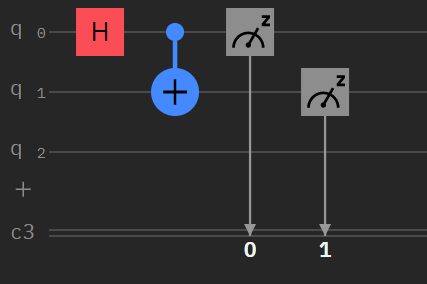
\includegraphics[width=\textwidth]{img/circuitVB.PNG}
        \caption{This is an example of a simple quantum circuit}
        \label{fig:Quantum circuit}
\end{figure}

\subsection{Gates}
\label{subsubsec:gates}
All the gates used in the composer will be explained first. All the information of the operations can be found on the website of IBM \footnote{$https://quantum-computing.ibm.com/composer/docs/iqx/operations_glossary$} on quantum computing as well as in \textcite{Hidary_2019} section 3.1 Quantum operators.
There are 5 types of gates: classicals, quantum's, phases, non-unitaries and the Hadamard gate. Most of the gates are reversible: when the same operation is used twice on a qubit, its state will be the same as the starting state \autocite{reversible_gates, revgates}.

The first gates that will be discussed are the classical gates, also known as Pauli gates. In this group 4 gates can be found: the NOT gate, the CNOT gate, the Toffoli gate and the SWAP gate.
In figure \ref{fig:classical gates} the representation of the classical gates in composer is given in the following order, NOT, CNOT, Toffoli and SWAP.
The not gate, or Pauli X gate, flips the state of a qubit. The controlled not gate, or CX, uses 2 qubits. One qubit is the target that will be flipped if the control qubit is in state $\ket{1}$. It can also function as an operation to make an entanglement.
In this case if the control qubit is in a superposition, both qubits will be entangled. The Toffoli gate acts as a double CNOT gate. It uses two controll qubits that have to be in the $\ket{1}$ state to flip the target.
Finally, there is the SWAP gate. This is self-explanatory because it just swaps the states of two qubits. There is a special gate called the identity gate. In fact, it's not a gate at all, this 'gate' is a blank unit in the gate time to ensure nothing can happen with that qubit at that exact moment.

\begin{figure} [h]
    \centering
    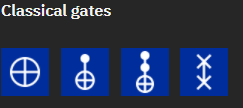
\includegraphics[width=\textwidth]{img/classical-gates.PNG}
        \caption{A visual representation of the classical gates \autocite{imggates}}
        \label{fig:classical gates}
\end{figure}

Next up are the phase gates. This group of gates exists of the T gate, S gate, Z gate, T$\dagger$ gate, S$\dagger$ gate, phase gate and the RZ gate, and are shown in figure \ref{fig:phase gates}. These gates shift the phase of the qubits.
The T$\dagger$ and S$\dagger$ gates are the inverse gates of the respectively T and S gate. And the T, S and Z gates are just 'special' cases of the phase gate.
In table \ref{tab:pgates} the matrix representation of each gate can be found.

\begin{figure} [h]
    \centering
    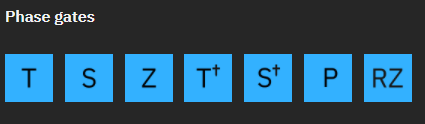
\includegraphics[width=\textwidth]{img/phase-gates.PNG}
        \caption{A visual representation of the phase gates \autocite{imggates}}
        \label{fig:phase gates}
\end{figure}

There are 5 different non-unitary operators or modifiers. These operators are reset, measurement, the control modifier, IF and the barrier operation as shown in figure \ref{fig:non-uni gates}.
The reset operations reset the qubit to the $\ket{0}$ state. This operation doesn't take any previous state into consideration and is not reversible.
The measurement operation also is not reversible and measures the qubit. So, its output gives the value of the qubit in the standard basis.
Applying an IF operation can give conditions to quantum gates. The conditions in the if operations depend on the state of the classical register, not the quantum one.
When a circuit is executed, the computer will try to combine gates to increase the efficiency. If these combinations should not happen, de barrier operation can be used.
The control modifier is used with another operation. Say for example the Z-gate is used and a control modifier is applied to that, the Z-gate will only be executed if the qubit on which the control lays is in state $\ket{1}$.

\begin{figure} [h]
    \centering
    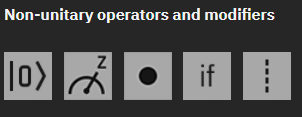
\includegraphics[width=\textwidth]{img/non-unitary-gates.PNG}
        \caption{A visual representation of the non-unitary gates \autocite{imggates}}
        \label{fig:non-uni gates}
\end{figure}

The Hadamard gate is used to make superpositions. When applying this gate to a qubit in state $\ket{1}$ or $\ket{0}$, it rotates it resulting respective states $\ket{-}$ and $\ket{+}$

\begin{figure} [h]
    \centering
    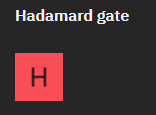
\includegraphics[width=\textwidth]{img/hadamard-gate.PNG}
        \caption{A visual representation of the hadamard gate \autocite{imggates}}
        \label{fig:hadamard gates}
\end{figure}

$\sqrt{X}$, $\sqrt{X}$$\dagger$, Y, RX, RY, RXX, RZZ and U make up the last set of gates: the quantum gates. 
The RX and RY respectively rotate the qubit around the x- and y-axis. The Y-gate is a special case of RY, where $\theta$ equals $\pi$.
Since the U gate takes in three angles as input, it can be used to make any gate as long as it's a single qubit gate.
$\sqrt{X}$ and it's inverse $\sqrt{X}$$\dagger$ can make a superposition if the qubit it is applied to is in state $\ket{0}$. If the gates are applied twice in a row the output will give a standard NOT-gate.
In table \ref{tab:qgates} a representation can be found on the matrixes of every quantum gate.

\begin{figure} [h]
    \centering
    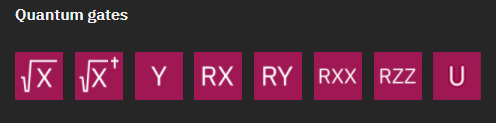
\includegraphics[width=\textwidth]{img/quantum-gates.PNG}
        \caption{A visual representation of the quantum gates \autocite{imggates}}
        \label{fig:quantum gates}
\end{figure}

\begin{table}[]
\label{tab:pgates}
\caption{Matrix representations of the phase gates.}
        \begin{tabular}{l|l}
        \hline
        \multicolumn{1}{|l|}{Phase Gate}  & \multicolumn{1}{l|}{Matrix representation of the gate}               \\ \hline
        T                                 & $\begin{pmatrix}1&0 \\ 0& \exp(i\frac{\theta}{4})\end{pmatrix}$      \\
        Z                                 & $\begin{pmatrix}1&0 \\ 0& -1\end{pmatrix}$                           \\
        S                                 & $\begin{pmatrix}1&0 \\ 0& i\end{pmatrix}$                            \\
        T$\dagger$                        & $\begin{pmatrix}1&0 \\ 0& \exp(-i\frac{\theta}{4})\end{pmatrix}$     \\
        S$\dagger $                       & $\begin{pmatrix}1&0 \\ 0& -i\end{pmatrix}$                           \\
        P                                 & $\begin{pmatrix}1&0 \\ 0& \exp(i\lambda)\end{pmatrix}$               \\
        RZ                                & $\begin{pmatrix}\exp(-i\frac{\lambda}{2})&0 \\ 0& \exp(i\frac{\lambda}{2})\end{pmatrix}$                                    
        \end{tabular} 
\end{table}
    
\begin{table}[]
    \label{tab:qgates}
    \caption{Matrix representations of the quantum gates.}
        \begin{tabular}{l|l}
        \hline
        \multicolumn{1}{|l|}{Phase Gate}  & \multicolumn{1}{l|}{Matrix representation of the gate}                                                                                                                                                                                                                         \\ \hline
        RX                                & $\begin{pmatrix} \cos\frac{\theta}{2}&-i\sin\frac{\theta}{2}              \\ -i\sin\frac{\theta}{2}&\cos\frac{\theta}{2}                                                                                                                                        \end{pmatrix}$ \\
        RY                                & $\begin{pmatrix} \cos\frac{\theta}{2}&-\sin\frac{\theta}{2}               \\ \cos\frac{\theta}{2}&\sin\frac{\theta}{2}                                                                                                                                          \end{pmatrix}$ \\
        RXX                               & $\begin{pmatrix} \cos\frac{\theta}{2}&0&0&-i\sin\frac{\theta}{2}          \\ 0&\cos\frac{\theta}{2}&-i\sin\frac{\theta}{2}&0                           \\ 0&-i\sin\frac{\theta}{2}&\cos\frac{\theta}{2}&0 \\ -i\sin\frac{\theta}{2}&0&0&\cos\frac{\theta}{2}    \end{pmatrix}$ \\                               
        RZZ                               & $\begin{pmatrix} \exp(-i\frac{\theta}{2})&0&0&0                           \\ 0&\exp(i\frac{\theta}{2})&0&0                                             \\ 0&0&\exp(i\frac{\theta}{2})&0 \\ 0&0&0&\exp(-i\frac{\theta}{2})                                       \end{pmatrix}$ \\         
        $\sqrt{X}$                        & $\begin{pmatrix} 1+i&1-i                                                  \\ 1-i&1+i                                                                                                                                                                            \end{pmatrix}$ \\
        $\sqrt{X}\dagger$                 & $\begin{pmatrix} 1-i&1+i                                                  \\ 1+i&1-i                                                                                                                                                                            \end{pmatrix}$ \\
        U                                 & $\begin{pmatrix} \cos\frac{\theta}{2}&-\exp(i\lambda)\sin\frac{\theta}{2} \\ \exp(i\phi)\sin\frac{\theta}{2}&\exp(i(\phi+\lambda))\cos\frac{\theta}{@}                                                                                                          \end{pmatrix}$ \\
        Y                                 & $\begin{pmatrix} 0&-i \\ i&0                                                                                                                                                                                                                                    \end{pmatrix}$                                   
        \end{tabular}
\end{table}

\section{Quantum lab}
\label{sec:Qlab}
Quantum lab is nothing more than a jupyter notebook wherein code is written. The only exception is that this code is run on a quantum computer instead of a classical computer.
To write quantum algorithms there is an open-source project called 'Qiskit'. This project is made by IBM and can be used on their quantum computer on the cloud. Using qiskit makes working on a quantum computer a bit easier.
It already has a great library of defined methods that can be used after importing the package. In this study the class Shor will be used to execute factoring with Shor's algorithm, so the algorithm itself should not be rewritten.
